\section{Attack overview}
\label{sec:attack}
We begin by summarizing our attack.  Our attack is based on traffic correlation,
so it requires an attacker to observe traffic that is both entering and exiting
the Tor network.  In contrast to earlier work, we consider DNS instead of just
end-to-end TCP packets.

Our attack is illustrated in Figure~\ref{fig:attack-scenario} and requires the
following building blocks:

\begin{figure}[t]
	\centering
	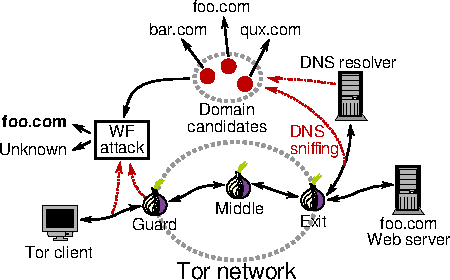
\includegraphics[width=\linewidth]{figures/attack-scenario.pdf}
	\caption{An overview of our correlation attack.  Ingress traffic is
	monitored either by a network-level adversary or the guard relay.  Egress
	traffic is monitored either by a network-level adversary or a DNS server.
	Captured DNS queries then serve as the candidate set for a Website
	fingerprinting attack.}
	\label{fig:attack-scenario}
\end{figure}

\begin{description}
	\item[Ingress sniffing] An attacker must observe traffic that is entering
		the Tor network.  The attacker can operate on the network level, i.e.,
		be a malicious ISP, or an intelligence agency.  In addition, the
		attacker can operate on the relay level, i.e., run a malicious Tor guard
		relay.  Note that in both cases, the attacker can only observe encrypted
		data.  Therefore, packet meta information such as packet lengths and
		directions serve as input to a website fingerprinting
		attack~\cite{Panchenko2016a}.
	\item[Egress sniffing] To observe both ends of the communication, an
		attacker must also observe egress DNS traffic.  We expect the adversary
		to operate on the network level, i.e., be on the path between exit relay
		and a DNS server.  Alternatively, the attacker can run a malicious DNS
		resolver or server.  Note that an attacker may also run an exit relay,
		but in that case she might as well do classical end-to-end correlation.
	\item[WF fingerprinting] We employ a website fingerprinting attack to
		determine if any of the recently observed DNS queries in egress traffic
		could be part of the encrypted ingress traffic.  Note that the DNS query
		itself does not tell us what \emph{page} a user is going to.
\end{description}

\subsection{Egress sniffing -- simulating Tor-exits' DNS traffic}
% the angle is: we have to simulate all DNS traffic from all Tor exits,
% the goal is to convince that we'ev made reasonable assumptions
To estimate the capability of an attacker, we need to investigate what
DNS data is observable for the attacker, that is what DNS request are
emerging from Tor exit relays.

We cannot use real data because there are no logs of outgoing traffic
from Tor exit relays available to us and ethical considerations kept us
from trying to collect them (\eg by operating exit relays and recording
the outgoing traffic). We therefore \emph{simulate} the DNS traffic
emerging from Tor exit relays.

\subsubsection{Website Popularity Distribution}
% powerlaw, not uniform
First, we model \emph{what websites} are visited by Tor users.
Currently, there are about 170 million active
websites\footnote{\url{http://news.netcraft.com/archives/2016/06/22/june-2016-web-server-survey.html}}
in the world and the Alexa ranking gives insights into their popularity
based on the browsing behaviour of a sample of all internet users
\footnote{\url{https://support.alexa.com/hc/en-us/articles/200449744}}.
It has been shown that the popularity of a website follows a powerlaw
distribution based on the rank of the website\fixme{citation needed}. So
we fit a powerlaw distribution to the page view numbers of the Alexa top
10\,000 websites\footnote{We used the python powerlaw package
		\url{https://github.com/jeffalstott/powerlaw} for fitting, the
		resulting powerlaw distribution had an $\alpha$ parameter of
		$1.10291152854$. Page view numbers as collected by Alexa ignore
		multiple visits by the same user on the same day, so the ranking
		might be slightly off for our purposes.} and use the result to
model which websites are visited by Tor users.
This might overestimate the popularity of higher-ranked websites because
Tor users might be visiting less popular websites, such as websites that
are censored in different parts of the world, more often than the
average internet users and we will discuss the implications of this for
our results later on.

\subsubsection{Page load frequency}
% phw's numbers extrapolated
Second, we determine \emph{how many websites} are visited by Tor users in a
certain time span. We use (less intrusive) statistics on the number of
outgoing DNS requests collected on a Tor exit relay under our control
and interpolate these numbers to all Tor exit relays based on the
published bandwidth statistics of all Tor exit relays\footnote{We found
		our exit relay \texttt{746BE73579F274AFEFA5E12C4ADACD53784D0762}
		to have on average 119.3 outgoing DNS requests per 5 minutes
		during a two week period, which corresponds to about 1.583 page
		visits per minute (taking caching into account and assuming a
		powerlaw distribution of site popularity as described above).
		The exit was configured to only allow port 80 and 443 during the
		time of the measurements to avoid counting DNS requests from
		other protocols than HTTP and HTTPS. We then used the
		self-reported bandwidth information from Tor exit relays
		collected in the ``extra-info'' descriptors available on
		\url{https://collector.torproject.org/} to estimate the number
		of page loads on each of the about 1200 exit relays active at
		that time.}.

\subsubsection{DNS caching}
% exit caching only (limitation: client-side caching negligible?)
To analyze which DNS requests can be seen by the adversary, we need to
take caching of DNS responses into account. We ignore client-side DNS
caching\footnote{The Tor browser, built on Mozilla Firefox, caches up to
		400 DNS entries internally for 60 seconds (config setting
		\texttt{network.dnsCacheExpiration} is set to 60,
		\texttt{network.dnsCacheEntries} is set to 400). The Tor client
		also maintains a local DNS cache based on responses from exits.
		 %Q: Does it respect TTLs or does it do clipping? A: it gets clipped since
		 % the response from the exit is already clipped.
			\fixme{is it activated by default?
				(CacheIPv4DNS is on by default, according to
				https://www.torproject.org/docs/tor-manual.html.en but I
				did not figure out if UseDNSCache is on by default?)}}
because in most cases the local cache entries expire before the user
re-visits the same website \fixme{How can we argue better here? maybe
		relate this to the Alexa-way of measuring page visits, ie.
		ignoring multiple visits of the same user on the same day?
		Is the cache active for different circuits? If not, then the caches are
		irrelevant due to our sliding window of DNS requests.}.
On the exit relays, where the actual DNS resolution takes place, caching
becomes more relevant as the requests of all users that choose a certain
exit relay for a connection will be handled by this exit relay. An exit
relay maintains its own DNS cache\footnote{Around eventdns.c.  See the
		code in src/or/dns.c.} and enforces a minimum TTL of 60 seconds
and a maximum TTL of 30 minutes\footnote{See src/or/dns.c:278}.  We
refer to this as Tor's \emph{TTL clipping}. Due to a
bug\footnote{\url{https://trac.torproject.org/projects/tor/ticket/19025}}
in Tor, the TTL of all DNS responses are set to 60 seconds.

%\subsubsection{Sliding window approach to compensate for DNS caching}
% we ignore caching by having a window of X minutes
If a user of an exit relay requests the IP address for a domain name
that has been cached by the exit relay before (and the cache entry is
not expired yet), then the adversary will not be able to observe an
outgoing DNS request for this domain name. But the adversary can
recorded all DNS requests from the exit relay in the past $x$ minutes,
where $x$ is the maximum TTL value (that is, maintain a sliding window of
size $x$) to obtain a list of all possibly requested domain names at the
given point in time. A domain name that is requested by a client at the
given point in time is either contained in the cache or not. If it is
not contained in the cache, it will be observable as a new, outgoing DNS
request from the exit relay. If it is contained in the cache it must
have been resolved by the exit relay in the last $x$ minutes and will
therefore be contained in the sliding window.

We assume that an adversary applies this sliding window technique and
model the observable DNS data accordingly. That is, we simulate a cache for
each exit relay: we trigger a page load event with a frequency
corresponding to the exit's bandwidth (see page load frequency above).
For each such page load event we randomly draw a website using the
powerlaw website popularity distribution described above. For all DNS
requests that are triggered by loading the chosen website we create a
new entry in the cache only if the domain name is not contained in the
cache yet and set the TTL for each entry to 60 seconds. At the end of
the simulation the content of the cache corresponds to the sliding
window that the adversary can observe because each non-expired entry in
the cache corresponds to a domain name that would have been resolved by
the exit relay during the past 60 seconds.


\subsubsection{DNS 1Mx5 dataset}
% TODO: pulls
% unique domain names are useful + TTL distribution (?)
TL;DR: unique domains are useful.

\subsubsection{A naive website classifier}
% TODO: whomever gets here first :-)
% we only look for unique domain names
% + naive, but already good enough for our purposes
% we note that we can significantly improve attacks by digging deeper
% into TTLs (even with window) and requests
In the end, we get a list of observed sites. We only look for sites that are
on the monitored list for the WF attack.
